\section{Evaluation}
\label{sec:evaluation}

Not available. Waiting for the dataset.

%Two standard metrics are used to measure the accuracy of prediction algorithms: \textit{area under the receiver operating characteristic curve} - AUC, and  \textit{Precision} \cite{Lu2011}.

%ARGOMENTARE LE METRICHE AUC E PRECISION
%ARGOMENTARE COME VENGONO GENERATI I TRAINING/TEST INTERVAL.

%\begin{figure}
%	\centering
%	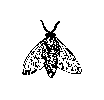
\includegraphics{./fig/fly}
%	\caption{AUC and Precision indices for link detection metric, considering both a criminal and a social network dataset.}
%	\label{fig:performance-detection}
%\end{figure}

%\begin{figure}
%	\centering
%	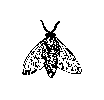
\includegraphics{./fig/fly}
%	\caption{AUC and Precision indices for link prediction metric, considering both a criminal and a social network dataset.}
%	\label{fig:performance-prediction}
%\end{figure}

% DA INSERIRE
%Formally, for two istants $t$ and $t' > t$, we denote $G[t,t']$ the subgraph of G consisting of all edges with a timestamp between $t$ and $t'$. Identified four times: $t_{0}, t'_{0}, t_{1}, t''_{1}$, with $t_{0}<t'_{0}<t_{1}<t'_{1}$, we refer to $[t_{0},t'_{0}]$ as the \textit{training interval} and $[t_{1},t'_{1}]$ as the \textit{test interval}. Applying a \textit{prediction algorithm} on the graph obtained after the training interval, as $G[t_{0},t'_{0}]$, we want to make a prediction on the edges that will be present in the graph $G[t_{1},t'_{1}]$ and not present in $G[t_{0},t'_{0}]$\cite{Liben-Nowell}.
%In this work, the notions of training interval and test interval, are provided with the only purpose to test the algorithm that will be presented in the following. After all, this application produce an output of links mining in real time: in which each instant $t\textsuperscript{*}>t_{0}$ identifies a graph $G[t_{0},t\textsuperscript{*}]$ on which to execute the algorithm. More details about the real time processing are explained in Section \ref{sec:architecture}.

%Notice that, in this work we assume that the graph is connected, therefore each pair of nodes is connected by a path. If we had in the case of a not connected graph, with a large connected component, as \textit{giant component}, and other small size connected components, the accuracy would be distorted by different \textit{density} of edges in a connected components.
